% siminos/xiong/thesis/chapters/ped.tex
% $Author: predrag $ $Date: 2017-04-03 11:00:42 -0400 (Mon, 03 Apr 2017) $

When studying the dimension of an inertial manifold in \refsect{sect:ksdim}, we have
used the information of the Floquet spectra and \Fv s of \ppo s and \rpo s.
In this chapter, we discuss how to calculate them accurately.

The Floquet matrix can be naively obtained numerically by
integrating \refeq{eq:tangentDynamics}
along the orbit.
However, it is almost certain that this process will overflow or
underflow at an exponential rates as the system evolves, or the
resulting Jacobian is highly ill-conditioned. Thus,
accurate calculation of expansion rate
is not trivial for nonlinear systems, especially for
those that evolve in high\dmn\ spaces. In such cases, the
expansion/contraction rates can easily range over many orders of magnitude,
which raises a challenge to formulating an effective algorithm to tackle this
problem. However, the semi-group property \refeq{eq:xjacobian} enables
us to factorize the \JacobianM\ into a
product of short-time matrices with matrix elements of
comparable orders of magnitude.
So the problem is reduced to calculating the eigenvalues of the product
of a sequence of matrices.

In this chapter, we introduce \ped\ algorithm, which is designed to calculate the
full Floquet spectrum and \Fv s. It is
based on the \cLv\ algorithm (\refsect{subsec:clvs}) and the \psd\
(\refsect{subsec:psd}).

\section{Description of the problem}
\label{sect:problem}

According to
\eqref{eq:xjacobian}, \JacobianM\ can be integrated piece by
piece along a state orbit:
\[
  \jMps^{\zeit}(\ssp_0) =
  \jMps^{\zeit_{m}-\zeit_{m-1}}(\ssp(\zeit_{m-1}) ,\zeit_{m-1})
  \cdots
  \jMps^{\zeit_{2}-\zeit_{1}}(\ssp(\zeit_{1}) ,\zeit_{1})
  \jMps^{\zeit_{1}-\zeit_{0}}(\ssp(\zeit_{0}) ,\zeit_{0})
\]
with $\zeit_{0}=0$, $\zeit_{m}=t$ and $\ssp_0$ the initial point. For \po s,
$\ssp(\zeit_{m}) = \ssp_0$.
The time sequence $t_i$, $i=1,2,\cdots, m-1$ is
chosen properly such that the elements of the
\JacobianM\ associated with each small time interval have a relatively
similar order of magnitude.
For simplicity, we drop all the parameters above and use a bold
letter to denote the product:
\begin{equation}
  \ps{\jMps}{0}=\jMps_{m}\jMps_{m-1}\cdots \jMps_{1}\,,\quad
  \jMps_{i}\in \mathbb{R}^{n\!\times\! n},\; i\!=\!1,2,\cdots,m
  \,.
  \label{eq:problem}
\end{equation}
Let the eigendecomposition of $\ps{\jMps}{0}$ be
\begin{equation}
  \label{eq:diagonal}
  \ps{\jMps}{0}=E^{(0)}\Sigma(E^{(0)})^{-1}
  \,,
\end{equation}
where $\Sigma$ is a diagonal matrix which stores $\ps{\jMps}{0}$'s
eigenvalues (Floquet multipliers),
$\{ \ExpaEig_{1}, \cdots, \ExpaEig_{n}\}$, and
columns of matrix $E^{(0)}$ are the eigenvectors (\Fv s)
of $\ps{\jMps}{0}$:
$E^{(0)}=[\Jve{1}, \cdots, \Jve{n}]$. In this chapter all
vectors are written in the column form, transpose of $v$ is denoted
$\transp{v}$, and Euclidean `dot' product by $(\transp{v}\,u)$. The
challenge associated with obtaining diagonalized form \eqref{eq:diagonal}
is the fact that often $\ps{\jMps}{0}$ should not be written
explicitly since the integration process \eqref{eq:tangentDynamics} may overflow
or the resulting matrix is highly ill-conditioned.
Floquet multipliers can easily vary over {hundreds of}
orders of magnitude,
depending on the system under study and the period of the orbit;
therefore, all transformations should be applied to the short-time
\JacobianMs\ $J_i$ individually, instead of working with the full-time
$\ps{\jMps}{0}$.
Also, in order to characterize
the geometry along a \po, not only the Floquet
vectors at the initial point are required, but also the
sets at each point on the orbit. Therefore, we also desire
the eigendecomposition of the cyclic rotations of $\ps{\jMps}{0}$:
$\ps{\jMps}{k}=\jMps_{k}\jMps_{k-1}\cdots \jMps_{1}\jMps_{m}\cdots
\jMps_{k+1}$ for $k=1,2,\dots,m\!-\!1$. Eigendecomposition of all
$\ps{\jMps}{k}$ is called the \emph{periodic eigendecomposition} of the
matrix sequence $\jMps_{m}, \jMps_{m-1}, \cdots ,\jMps_{1}$.

The process of implementing eigendecomposition \eqref{eq:diagonal}
proceeds in two stages. First, {\prsf} (PRSF) is
obtained by a similarity transformation for each $\jMps_i$,
\begin{equation}
  \label{eq:prsf}
  \jMps_{i}=Q_{i}R_{i}Q_{i-1}^\top
  \,,
\end{equation}
with $Q_{i}$ orthogonal matrix, and $Q_{0}=Q_{m}$.
{One of $R_i$ above is quasi-upper triangular with
  $[1\!\times\! 1]$ and $[2\!\times\! 2]$ blocks on the
  diagonal, and the others are all upper triangular. Since the definition
  of $\ps{\jMps}{k}$ is cyclic, we can choose $R_m$ to be
  quasi-upper triangular without loss of generality.}
The existence of PRSF, proved in
\refref{Bojanczyk92theperiodic}, provides the \pqr\ that implements \psd.
Defining $\ps{R}{k}=R_{k}R_{k-1}\cdots R_{1}R_{m}\cdots R_{k+1}$, we have
\begin{equation}
  \label{eq:pedrotation}
  \ps{\jMps}{k}=Q_{k}\ps{R}{k}Q_{k}^\top
  \,,
\end{equation}
with the eigenvectors of matrix $\ps{\jMps}{k}$ related to eigenvectors
of quasi-upper triangular matrix $\ps{R}{k}$ by orthogonal matrix
$Q_{k}$. $\ps{\jMps}{k}$ and $\ps{R}{k}$ have the same eigenvalues,
stored in the $[1\!\times\! 1]$ and $[2\!\times\! 2]$ blocks on the
diagonal of $\ps{R}{k}$, and their eigenvectors are transformed by
$Q_{k}$, so the second stage concerns the eigendecomposition of
$\ps{R}{k}$. Eigenvector matrix of $\ps{R}{k}$ has the same structure as
$R_{m}$. We evaluate it by two distinct algorithms. The first one is power
iteration, while the
second algorithm relies on solving a \pse\rf{GranatK06}.

As all $\ps{R}{k}$ have the same eigenvalues, and their eigenvectors are
related by similarity transformations,
\begin{equation}
  \label{eq:Rrelation}
  \ps{R}{k}=(R_{m}\cdots R_{k+1})^{-1}\ps{R}{0}(R_{m}\cdots R_{k+1})
  \,,
\end{equation}
one may be tempted to calculate the eigenvectors of $\ps{R}{0}$, and
obtain the eigenvectors of $\ps{R}{k}$ by \eqref{eq:Rrelation}. The
pitfall of this approach is that numerical errors accumulate when
multiplying a sequence of upper triangular matrices, especially for large
$k$, {such that contracting eigenvectors are contaminated by expanding
  ones during this process}.

Our work illustrates the connection between different algorithms in the
two stages of implementing \ped, pays attention to the case when
eigenvectors appear as complex pairs, and demonstrates that eigenvectors
can be obtained directly from \pse\ without restoring PRSF.


\section{Stage 1 :  periodic real Schur form (PRSF)}
\label{sect:psd}
This is the first stage of implementing \ped.
Eq.~\eqref{eq:pedrotation} represents the eigenvalues of matrix
$\ps{\jMps}{k}$ as real eigenvalues on the diagonal, and complex
eigenvalue pairs as $[2\!\times\! 2]$ blocks on the diagonal of
$\ps{R}{k}$. More specifically, if the $i$th
eigenvalue is real, it is given by the product of all the $i$th
diagonal elements of matrices $R_{1},R_{2},\cdots,R_{m}$. In practice,
the logarithms of magnitudes of these numbers are added, in order to
overcome numerical {overflow or underflow}. If the $i$th and $(i+1)$th
eigenvalues form a complex conjugate pair, all $[2\!\times\! 2]$ matrices
at position $(i,i+1)$ on the diagonal of $R_{1},R_{2},\cdots,R_{m}$ are
multiplied with normalization at each step, and the two complex
eigenvalues of the product are obtained. There is no danger of numerical
{overflow or underflow}
because all these $[2\!\times\! 2]$  matrices are in the same
position and  in our applications their elements are of similar order of
magnitude.
\refSect{subsec:psd} introduces the \psd\ to achieve PRSF. An
alternative is the first two stages of {\cLv\ algorithm} in \refsect{subsec:clvs},
which reduces to simultaneous iteration for \po s.
{Actually, for a single matrix,
  simultaneous iteration is equivalent to $QR$ iteration\rf{Trefethen97}.
  When it comes to matrix product, simultaneous iteration and \psd\ both
  achieve the PRSF, but their computational complexities differ.}

\paragraph{Simultaneous iteration}

The basic idea of simultaneous iteration is implementing QR decomposition
in the process of power iteration. Assume all Floquet multipliers
are real, without degeneracy, and order them by their
magnitude: $|\ExpaEig_{1}|>|\ExpaEig_{2}|>\cdots >|\ExpaEig_{n}|$, with
corresponding normalized \Fv s
$\jEigvec[1], \jEigvec[2],\cdots, \jEigvec[n]$.
For simplicity, here we have dropped the upper indices of these vectors.
An arbitrary initial vector
$\tilde{q}_{1}=\sum_{i=1}^{n}\alpha^{(1)}_{i}\jEigvec[i]$ will converge to the
first \Fv\ $\jEigvec[1]$ after normalization under power iteration of
$\ps{\jMps}{0}$,
\[
  \lim_{\ell\to \infty }\frac{(\ps{\jMps}{0})^{\ell}\tilde{q}_{1}}{||\cdot||}
  \to q_{1}=\jEigvec[1]
  \,.
\]
Here $||\cdot||$ denotes the Euclidean norm of the numerator
($||x||=\sqrt{x^\top x}$). Let $\langle a,b,\cdots,c\rangle$ represent
the space spanned by vector $a,b,\cdots,c$ in $\mathbb{R}^n$. Another
arbitrary vector $\tilde{q}_{2}$ is then chosen orthogonal to subspace
$\langle q_{1} \rangle$ by Gram-Schmidt orthonormalization,
$\tilde{q}_{2}= \sum_{i=2}^{n}\alpha^{(2)}_{i}[\jEigvec[i]-(q_{1}^\top
\jEigvec[i])q_{1}]$.
Note that the index starts from $i=2$ because $\langle q_{1}
\rangle=\langle {\jEigvec[1]} \rangle$. The strategy now is to apply power
iteration of $\ps{\jMps}{0}$ followed by orthonormalization in each
iteration.
\begin{align*}
  \ps{\jMps}{0}\tilde{q}_{2}= &\sum_{i=2}^{n}\alpha^{(2)}_{i}
                                [\ExpaEig_{i}\jEigvec[i]-\ExpaEig_{1}(q_{1}^\top \jEigvec[i])q_1]
                                = \sum_{i=2}^{n}\alpha^{(2)}_{i}\ExpaEig_{i}[\jEigvec[i]-
                                (q_{1}^\top \jEigvec[i])q_{1}]+\sum_{i=2}^{n}\alpha^{(2)}_{i}
                                (\ExpaEig_{i}-\ExpaEig_{1})(q_{1}^\top \jEigvec[i])q_{1}
                                \,.
\end{align*}
The second term in the above expression will disappear after performing
Gram-Schmidt orthonormalization to $\langle q_{1} \rangle$, and the first
term will converge to
$q_{2}=\jEigvec[2]-(q_{1}^\top \jEigvec[2])q_{1}$ (not
normalized) after a sufficient number of iterations because of the
descending magnitudes of $\ExpaEig_{i}$, and we also note that $\langle
{\jEigvec[1], \jEigvec[2]} \rangle=\langle q_{1}, q_{2}\rangle$. The same argument can
be applied to $\tilde{q}_{i},\;i=3,4,\cdots,n$ as well.
In this way, after a sufficient number of iterations,
\[
  \lim_{\ell\to \infty}(\ps{\jMps}{0})^{\ell}[\tilde{q}_{1},\tilde{q}_{2},\cdots,
  \tilde{q}_{n}]
  \to [q_{1},q_{2}\cdots, q_{n}]
  \:,
\]
where
\[
  \begin{aligned}
    & q_{1} = \jEigvec[1]\,,\qquad
    q_{2} = \frac{\jEigvec[2]-(\jEigvec[2]^\top q_{1})q_{1}}{||\cdot ||}\,,
    \quad \cdots\,,\quad
    q_{n} = \frac{\jEigvec[n]-\sum_{i=1}^{n-1}(\jEigvec[n]^\top
      q_{i})q_{i}}{||\cdot ||}
    \,.
  \end{aligned}
\]
Let matrix $Q_{0}=[q_{1},q_{2},\cdots ,q_{n}]$; then we have
$\ps{\jMps}{0}Q_{0}=Q_{0}\ps{R}{0}$ with $\ps{R}{0}$ an upper triangular
matrix because of $\langle q_{1},q_{2},\cdots,q_{i} \rangle=\langle
{\jEigvec[1], \jEigvec[2], \cdots,  \jEigvec[i]} \rangle$, which is just
$\ps{\jMps}{0}=Q_{0}\ps{R}{0}Q^\top_{0}$ (the Schur decomposition of
$\ps{\jMps}{0}$). The diagonal elements of $\ps{R}{0}$ are the
eigenvalues of $\ps{\jMps}{0}$ in decreasing order.
Numerically, the process described above can be implemented on an
arbitrary initial full rank matrix $\tilde{Q}_0$ followed by QR
decomposition at
{each step
  \begin{equation}
    \label{eq:qr}
    \jMps_{s}\tilde{Q}_{s-1}=\tilde{Q}_{s}\tilde{R}_{s}
  \end{equation}
  with}
$s=1,2,3,\cdots$ and $\jMps_{s+m}=\jMps_{s}$. For a sufficient number of
iterations, $\tilde{Q}_{s}$ and $\tilde{R}_{s}$ converge to $Q_{s}$ and
$R_{s}$ in \eqref{eq:prsf} for $s=1,2,\cdots,{m}$, so we achieve
\eqref{eq:pedrotation} the \psd\ of $\ps{\jMps}{k}$.

We have thus demonstrated that simultaneous iteration converges to
PRSF for real non-degenerate eigenvalues.
For complex eigenvalue pairs, the algorithm converges in the sense that
the subspace spanned by a complex conjugate vector pair converges. So,
\begin{equation}
  \label{eq:simcplx}
  \ps{\jMps}{0}Q_{0}=Q^{'}_{0}\ps{R}{0}=Q_{0}D\ps{R}{0}
  \,,
\end{equation}
where $D$ is a block-diagonal matrix with diagonal elements $\pm 1$
(corresponding to real eigenvalues) or $[2\!\times\! 2]$ blocks
(corresponding to complex eigenvalue pairs). Absorb $D$ into $R_{m}$,
then $R_{m}$ becomes a quasi-upper triangular matrix, and \eqref{eq:prsf}
still holds.
{Here, we focus on $Q_0$ instead of $Q_1,\cdots,Q_{m-1}$ because we
  assume $R_m$ is quasi-upper triangular in \eqref{eq:prsf}}.


\section{Stage 2 : eigenvector algorithms}
\label{sect:eigenvec}

Upon achieving PRSF,
the eigenvectors of $\ps{\jMps}{k}$ are related to the eigenvectors of
$\ps{R}{k}$ by orthogonal matrix $Q_{k}$ from \eqref{eq:prsf}, and
the
eigenvector matrix of $\ps{R}{k}$ has the same quasi-upper triangular
structure as $R_m$. In addition, if we follow the
simultaneous iteration method or
implement \psd\ without shift, eigenvalues are ordered by their
magnitudes on the diagonal. Power iteration utilizing this property
could be easily implemented to generate the eigenvector
matrix. This is the basic idea of the first algorithm for generating
eigenvectors of $\ps{R}{k}$, corresponding to the 3rd and 4th stage in
{\cLv\ algorithm} in \reffig{fig:CLV}.
Alternatively,
observation that
the first eigenvector of $\ps{R}{k}$ is trivial if it is real,
$\Rve{1}=(1,0,\cdots,0)^\top $, inspires us to reorder the
eigenvalues so that the $j$th eigenvalue is in the first diagonal
place of $\ps{R}{k}$; in this way, the $j$th eigenvector is obtained.
For both methods, attention should be paid to the complex conjugate
eigenvector pairs. In this section, $\Rve{i}^{(k)}$
denotes the $i$th eigenvector of $\ps{R}{k}$, contrast to
$\jEigvec[i]^{(k)}$
the eigenvectors of $\ps{J}{k}$, and for most cases, the upper indices
are dropped if no confusion occurs.

\subsection{Iteration method}

The prerequisite for iteration method is that all the eigenvalues are
ordered in an ascending or descending way by their magnitude on the
diagonal of $\ps{R}{k}$. Assume that they are in descending order, which
is the outcome of simultaneous iteration; therefore, the diagonal elements
of $\ps{R}{k}$ are $\ExpaEig_{1},\ExpaEig_{2},\cdots,\ExpaEig_{n}$, with
magnitudes from large to small.
If the $i$th eigenvector of $\ps{R}{k}$ is real, then it has form
$\Rve{i}=(a_{1},a_{2},\allowbreak \cdots,a_{i},0,\cdots, 0)^\top $. An arbitrary
vector whose first $i$ elements are non-zero
$x=(b_{1},b_{2},\cdots,b_{i},0, \allowbreak \cdots, 0)^\top $ is a linear combination
of the first $i$ eigenvectors: $x=\sum_{j=1}^{i}\alpha_{j}\Rve{j}$.
Use it as the initial condition for the power iteration by
$(\ps{R}{k})^{-1}=R_{k+1}^{-1}\cdots R_{m}^{-1}R_{1}^{-1}R_{2}^{-1}\cdots
R_{k}^{-1}$ and after a sufficient number of iterations,
\begin{equation}
  \label{eq:invpower}
  \lim_{\ell\to \infty} \frac{(\ps{R}{k})^{-\ell}x}{||\cdot||}=\Rve{i}
  \,.
\end{equation}
The property we used here is that $(\ps{R}{k})^{-1}$ and $\ps{R}{k}$ have
the same eigenvectors but inverse eigenvalues.
{Moreover, matrix
  sequence $R_{k+1}^{-1}\cdots R_{m}^{-1}R_{1}^{-1}R_{2}^{-1}\cdots R_{k}^{-1}$
  is applied sequentially in \eqref{eq:invpower},
  so if the $i$th eigenvector $\Rve{i}^{(k)}$
  of $(\ps{R}{k})^{-1}$ converges,
  then the $i$th eigenvector of $(\ps{R}{k-1})^{-1}$ is
  obtained by $\Rve{i}^{(k-1)}=R^{-1}_k\Rve{i}^{(k)}$ (need to be normalized).
  Therefore, the $i$th eigenvectors
  of $(\ps{R}{k})$ for $k=0, 1, \cdots, m$ are obtained almost
  simultaneously. Note, there is no numerical instability here as in
  \eqref{eq:Rrelation} because \eqref{eq:invpower} finds the
  most expanding direction in the subspace that only the first
  $i$ elements are non-zero}.

For a $[2\!\times\! 2]$ block on the diagonal of $\ps{R}{k}$, the
corresponding conjugate complex eigenvectors form a two\dmn\ subspace.
Any real vector selected from this subspace will rotate under power
iteration. In this case, power iteration still converges in the sense
that the subspace spanned by the complex
conjugate eigenvector pair converges.
Suppose the $i$th and $(i+1)$th eigenvectors of $\ps{R}{k}$ form a
complex pair. Two arbitrary vectors $x_{1}$ and $x_{2}$ whose first $i+1$
elements are non zero can be written as the linear superposition of the
first $i+1$ eigenvectors,
$x_{1,2}=(\sum_{j=1}^{i-1}\alpha^{(1,2)}_{j}\Rve{j})+\alpha^{(1,2)}_{i}\Rve{i}+
(\alpha^{(1,2)}_{i}\Rve{i})^{*}
$,
where $(*)$ denotes the complex conjugate. As for the real case, the
first $i\!-\!1$ components will vanish after a sufficient number of
iterations. Denote the two vectors at this instance to be $X_{1, 2}$
and form matrix $X=[X_{1},X_{2}]$.
The subspace spanned by $X_{1,2}$ does not change and $X$ will be rotated
after another iteration,
\begin{equation}
  (\ps{R}{k})^{-1}X=X^{'}=XC
  \,,
  \label{eq:similar}
\end{equation}
where $C$ is a $[2\!\times\! 2]$ matrix which has two complex conjugate
eigenvectors $\Rve{C}$ and $(\Rve{C})^{*}$. Transformation
\eqref{eq:similar} relates the eigenvectors of $\ps{R}{k}$ with those of
$C$: $[\Rve{i},(\Rve{i})^{*}]=X[\Rve{C},(\Rve{C})^{*}]$.
In practice, matrix $C$ can be computed by QR decomposition; let
$X=Q_{X}R_{X}$ be the QR decomposition of $X$, then
$C=R_{X}^{-1}Q_{X}^\top X^{'}$.
On the other hand,
complex eigenvectors are not uniquely determined in the sense that
$e^{i\theta}\Rve{i}$ is also an eigenvector with the same eigenvalue
as $\Rve{i}$ for an arbitrary {phase} $\theta$, so when comparing
results from different eigenvector algorithms, we need a constraint to
fix the phase of a complex eigenvector, such as letting the first element
be real.

We should note that the performance of power iteration depends on the ratios
of magnitudes of eigenvalues, so performance is poor for systems with
clustered eigenvalues. We {anticipate that proper modifications,
  such as shifted iteration or inverse iteration\rf{Trefethen97}, may help
  improve the performance}.
Such techniques are beyond the scope of this paper.

\subsection{Reordering method}
\label{sect:reorder}

There exists a direct algorithm to obtain the eigenvectors of every
$\ps{R}{k}$ at once without iteration. The idea is very simple: the
eigenvector corresponding to the first diagonal element of an
upper-triangular matrix is $\Rve{1}=(1,0,\cdots,0)^\top $. By
reordering the diagonal elements (or $[2\!\times\! 2]$ blocks) of
$\ps{R}{0}$, we can find any eigenvector by positioning the corresponding
eigenvalue in the first diagonal position. Although in our application
only reordering of $[1\!\times\! 1]$ and $[2\!\times\! 2]$ blocks is
needed, we recapitulate here the general case of reordering two adjacent
blocks of a quasi-upper triangular matrix following
Granat {\etal}\rf{GranatK06}.
Partition $R_{i}$ as
\[
  R_{i}=
  \left[
    \begin{array}{c|cc|c}
      R^{00}_{i} & * & *& * \\ \hline
      0 & R^{11}_{i} & R^{12}_{i} & * \\
      0 & 0 & R^{22}_{i} & * \\ \hline
      0 & 0 & 0 & R^{33}_{i}
    \end{array}
  \right]
  \,,
\]
where $R^{00}_{i}, R^{11}_{i},R^{22}_{i},R^{33}_{i}$ have size
$[p_{0}\!\times\! p_{0}], [p_{1}\!\times\! p_{1}], [p_{2}\!\times\!
p_{2}]$ and $[p_{3}\!\times\! p_{3}]$ respectively, and
$p_{0}+p_{1}+p_{2}+p_{3}=n$. In order to exchange the middle two blocks
($R^{11}_{i}$ and $R^{22}_{i}$), we construct a non-singular periodic
matrix sequence: $\hat{S_{i}},\:i=0,1,2,\cdots,m$ with
$\hat{S_{0}}=\hat{S}_{m}$,
\[
  \hat{S_{i}}=
  \left[
    \begin{array}{c|c|c}
      I_{p_{0}} & 0 & 0  \\ \hline
      0 & S_{i} & 0 \\ \hline
      0 & 0 & I_{p_{3}}
    \end{array}
  \right]
  \,,
\]
where $S_{i}$ is a $[(p_{1}+p_{2})\!\times\! (p_{1}+p_{2})]$ matrix,
such that $\hat{S}_{i}$ transforms $R_{i}$ as follows:
\begin{equation}
  \label{eq:xdtransform}
  \hat{S}_{i}^{-1}R_{i}\hat{S}_{i-1}=\tilde{R}_{i}=
  \left[
    \begin{array}{c|cc|c}
      R^{00}_{i} & * & *& * \\ \hline
      0 & R^{22}_{i} & 0 & * \\
      0 & 0 & R^{11}_{i} & * \\ \hline
      0 & 0 & 0 & R^{33}_{i}
    \end{array}
  \right]
  \,,
\end{equation}
which is
\[
  S^{-1}_{i}
  \left[
    \begin{array}{c c}
      R^{11}_{i} & R^{12}_{i} \\
      0 & R^{22}_{i}
    \end{array}
  \right]
  S_{i-1}=
  \left[
    \begin{array}{c c}
      R^{22}_{i} & 0 \\
      0 & R^{11}_{i}
    \end{array}
  \right]
  \,.
\]
The problem is to find the appropriate matrices $S_{i}$ which satisfy
the above condition. Assume $S_{i}$ has form
\[
  S_{i}=
  \left[
    \begin{array}{c c}
      X_{i} & I_{p_{1}} \\
      I_{p_{2}} & 0
    \end{array}
  \right]
  \,,
\]
where matrix $X_{i}$ has dimension $[p_{1}\!\times\! p_{2}]$. We obtain
periodic Sylvester equation\rf{GranatK06}
\begin{equation}
  \label{eq:xdpse}
  R^{11}_{i}X_{i-1}-X_{i}R^{22}_{i}=-R^{12}_{i}
  \,,\quad i=0,1,2,\cdots,m
  \,.
\end{equation}

The algorithm to find eigenvectors is based on \eqref{eq:xdpse}. If the
$i$th eigenvalue of $\ps{R}{k}$ is real, we only need to exchange the
{leading} $[(i-1)\!\times\! (i-1)]$ block of $R_{k}\,,k=1,2,\cdots,m$ with
its $i$th diagonal element. If the $i$th and $(i+1)$th
eigenvalues form a complex conjugate pair,
then the {leading} $[(i-1)\!\times\! (i-1)]$
block and the following $[2\!\times\! 2]$ block should be exchanged.
Therefore $X_{i}$ in \eqref{eq:xdpse} has dimension $[p_{1}\!\times\! 1]$
or $[p_{1}\!\times\! 2]$. In both cases, $p_{0}=0$.

\paragraph{Real eigenvectors}
In this case, matrix $X_{i}$ is just a column vector, so
\eqref{eq:xdpse} is equivalent to
\begin{equation}
  \label{eq:xdpsereal}
  \begin{bmatrix}
    R^{11}_{1} & -R^{22}_{1}I_{p_{1}} &  & \\[1em]
    & R^{11}_{2} & -R^{22}_{2}I_{p_{1}} &  &\\[1em]
    &  & R^{11}_{3} & -R^{22}_{3}I_{p_{1}} &  &\\[1em]
    & & & \ddots &\cdots & \\[1em]
    -R^{22}_{m}I_{p_{1}} & & & & R^{11}_{m}
  \end{bmatrix}
  \begin{bmatrix}
    X_{0} \\[1em]
    X_{1}  \\[1em]
    X_{2}  \\[1em]
    \cdots \\[1em]
    X_{m-1}
  \end{bmatrix}
  =
  \begin{bmatrix}
    -R^{12}_{1} \\[1em]
    -R^{12}_{2} \\[1em]
    -R^{12}_{3} \\[1em]
    \cdots \\[1em]
    -R^{12}_{m}
  \end{bmatrix}
  \,,
\end{equation}
where $R^{22}_{i}$ is the $(p_{1}+1)$th diagonal element of $R_{i}$.
The accuracy of eigenvectors is determined by the accuracy of
solving sparse linear equation \eqref{eq:xdpsereal}. In our application
to \po s in the one\dmn\ \KSe, \Gepp\ is enough. For a more
technical treatment, such as cyclic reduction or preconditioned conjugate
gradients, to name a few, please see\rf{NLA:NLA198,aabdls,GranatRBA}.

Now we get all vectors $X_{i}$ by solving \pse, but how are they related
to the eigenvectors? In analogy to $\ps{R}{0}$, defining
$\mathbf{\tilde{R}}_{0}=\tilde{R}_{m}\tilde{R}_{m-1}\cdots
\tilde{R}_{1}$, we get
$\hat{S}_{m}^{-1}\ps{R}{0}\hat{S}_{m}=\mathbf{\tilde{R}}_{0}$ by
\eqref{eq:xdtransform}. Since $p_{0}=0$ and $p_{2}=1$ in
\eqref{eq:xdtransform}, the first eigenvector of
$\mathbf{\tilde{R}}_{0}$, the one corresponding to eigenvalue
$\ExpaEig_{p_1+1}$
is $\tilde{e}=(1,0,\cdots , 0)^\top $. Apart from
normalization, the corresponding eigenvector of $\ps{R}{0}$ is
\[
  \Rve{p_{1}+1}^{(0)}=\hat{S}_{m}\tilde{e}
  = \left[X_{0}^\top , 1, 0, 0, \cdots, 0 \right]^\top
  \,.
\]
This is the eigenvector of matrix $\ps{R}{0}=R_{m}R_{m-1}\cdots R_{1}$ in
\eqref{eq:pedrotation} for $k=0$. For $\ps{R}{1}=R_{1}R_{m}\cdots R_{2}$,
the corresponding \pse\ will be cyclically rotated one row up {in
  \eqref{eq:xdpsereal}, which means $X_{1}$ will be shifted to the first
  place, and thus the corresponding eigenvector of}
$\ps{R}{1}$ is $\Rve{p_{1}+1}^{(1)}=[X_{1}^\top,1,0,\cdots,0]^\top $. The
same argument goes for all the {remaining $\ps{R}{k}$.}
In conclusion, solution of \eqref{eq:xdpsereal} contains the eigenvectors
for all $\ps{R}{k}\,,k=0,1,\cdots,m-1$.
Another benefit of reordering method is that we can selectively
get the eigenvectors corresponding to some specific eigenvalues.
This merit is important in high\dmn\ nonlinear systems for
which only a subset of \Fv s suffices to characterize the
dynamics in tangent space, and thus we avoid wasting time in calculating
{the remaining unimportant subset}.

\paragraph{Complex eigenvector pairs}
As in the real eigenvalue case, we have $p_{0}=0$, but now $p_{2}=2$, so
matrix $X_{i}$  has dimension $[p_{1}\!\times\! 2]$. Using the same
notation as \refref{GranatK06}, let $v(X_{i})$ denote the vector
representation of $X_{i}$ with the columns of $X_{i}$ stacked on top of
each other, and let $A\otimes B$ denote the Kronecker product of two
matrices, with the $(i,j)$-block element be $a_{ij}B$.

Now, the \pse\ \eqref{eq:xdpse} is equivalent to
\begin{equation}
  \label{eq:xdpsdcomplex}
  \resizebox{\linewidth}{!}{%
    $
    \setlength{\arraycolsep}{3pt}
    \begin{bmatrix}
      I_{2}\otimes R^{11}_{1} & -(R^{22}_{1})^\top \otimes I_{p_{1}} &  & \\[1em]
      & I_{2}\otimes R^{11}_{2} & -(R^{22}_{2})^\top  \otimes I_{p_{1}} &  &\\[1em]
      &  & I_{2}\otimes R^{11}_{3} & -(R^{22}_{3})^\top \otimes I_{p_{1}} &  &\\[1em]
      & & & \ddots &\cdots & \\[1em]
      -(R^{22}_{m})^\top \otimes I_{p_{1}} & & & & I_{2}\otimes R^{11}_{m}
    \end{bmatrix}
    \begin{bmatrix}
      v(X_{0}) \\[1em]
      v(X_{1})  \\[1em]
      v(X_{2})  \\[1em]
      \cdots \\[1em]
      v(X_{m-1})
    \end{bmatrix}
    =
    \begin{bmatrix}
      -v(R^{12}_{1}) \\[1em]
      -v(R^{12}_{2}) \\[1em]
      -v(R^{12}_{3}) \\[1em]
      \cdots \\[1em]
      -v(R^{12}_{m})
    \end{bmatrix} $%
  }
  \,.
\end{equation}
After switching $R^{11}_{i}$ and $R^{22}_{i}$, we can get the first two
eigenvectors of $\mathbf{\tilde{R}}_{0}$ by multiplying the first
$[2\!\times\! 2]$ diagonal blocks of $\tilde{R_{i}}$:
$R^{22}=R^{22}_{m}R^{22}_{m-1}\cdots R^{22}_{1}$. Let the eigenvectors of
$R^{22}$ be $v$ and $v^{*}$ of size $[2\!\times\! 1]$, then the
corresponding eigenvectors of $\mathbf{\tilde{R}}_{0}$ are
$\tilde{e}_{1}=(v^\top,0,0,\cdots,0)^\top $ and
$\tilde{e}_{2}=(\tilde{e}_{1})^{*}$ (the additional zeros make the length
of the eigenvectors be $n$). Therefore, the corresponding eigenvectors
of $\ps{R}{0}$ are
\[
  \left[\Rve{p_{1}+1}^{(0)},\Rve{p_{1}+2}^{(0)}\right]
  =\hat{S}_{m}[\tilde{e}_{1},\tilde{e}_{2}]
  = \left[
    \begin{array}{c}
      X_{0} \\
      I_{2}    \\
      0 \quad 0\\
      0 \quad 0\\
      \vdots\\
      0 \quad 0
    \end{array}
  \right]
  [v,v^{*}]
  \,.
\]
For other $\ps{R}{k}$, the same argument in the real case applies
here too, so we obtain all the complex eigenvector pairs for
$\ps{R}{k}\,,k=1,2,\cdots,m$.


\section{Computational complexity and convergence analysis}
\label{sect:error}

In this section, we make no attempt at conducting a strict error analysis of
the algorithms presented. However, for practical applications,
it is important to understand their computational costs.
\Ped\ is conducted in two stages: (1) {PRSF},
and (2) determination of all
eigenvectors. In each stage, there are two candidate algorithms, so the
efficiency of \ped\ depends on the choice of the specific algorithm
chosen in each stage.

\Psd\ algorithm and simultaneous iteration are both effective to achieve
PRSF. We estimate the complexity of \psd\ algorithm in analogy
with the single matrix case.
For a single $[n\!\times\! n]$ matrix, $O(n^3)$
flops (floating-point operations) are required\rf{Trefethen97}
to reduce it to upper Hessenberg form.
Accordingly, the first stage in
\reffig{fig:PSD} takes $O(mn^3)$ flops.
Then the implicit $QR$ iteration process for a single matrix
takes $O(n^2)$ flops for
a single iteration, so each iteration of the second stage in
\reffig{fig:PSD} takes $O(mn^2)$ flops.
Usually, the number of iterations exceeds by far the
dimension of the matrix. Therefore,  the average complexity of one
iteration in \psd\ algorithm is $O(mn^2)$. For a detailed discussion
see\rf{Bojanczyk92theperiodic, Trefethen97}.
On the other hand, simultaneous iteration
\eqref{eq:qr} requires
$m$ QR decomposition $O(mn^{3})$ and $m$ matrix-matrix multiplication
$O(mn^{3})$ in each iteration, giving a total computational cost of
$O(mn^{3})$. {Moreover, the convergence of both algorithms} depends
linearly on the ratio of adjacent eigenvalues of $\ps{R}{0}$:
$|\ExpaEig_{i}|/|\ExpaEig_{i+1}|$  without shift\rf{Francis61}.
Therefore,
the ratio of costs between \psd\ algorithm and simultaneous iteration
is approximately of the order $O(mn^2)/O(mn^3) = O(1/n)$,
implying that the \psd\ algorithm is much cheaper than the
simultaneous iteration if the dimension of matrices involved is large.

The second stage of \ped\ is to find all the eigenvectors of
$\ps{\jMps}{k}$ via quasi-upper triangular matrices $\ps{R}{k}$. The
first candidate is power iteration.
The computational cost of one iteration \eqref{eq:invpower} for the $i$th
eigenvector is $O(mi^{2})$. The second candidate, reordering method,
relies on an effective method to solve \pse\ \eqref{eq:xdpse}. For
example, \Gepp\ is suitable
for well-conditioned matrix \eqref{eq:xdpsereal} and
\eqref{eq:xdpsdcomplex} with a computational cost of $O(mi^{2})$
for the $i$th eigenvector. Here, we have taken account of
the sparse structure of \eqref{eq:xdpsereal} and
\eqref{eq:xdpsdcomplex}. For a detailed discussion, see \refref{GranatK06}.
So, the total complexity of reordering method is approximately the same as
that of one iteration in power iteration.

In summary, if we only consider the computational complexity,
the combination
of \psd\ algorithm and reordering method is preferable for \ped.

\section{Application to \KSe}
\label{sect:applic}

Our ultimate goal of implementing \ped\ is to analyze the stability
of \po s and the associated stable/unstable manifolds in
dynamical systems, for the hope of getting a better understanding
of pattern formation and turbulence.
As an example, we focus on the one\dmn\ \KSe \refeq{eq:ks}
and its Fourier space form \refeq{eq:ksfourier}. We follow
\refsect{sect:ksnumer} to integrate this system. For the
calculation of Floquet spectrum and vectors,
we use the combination of \psd\ algorithm and reordering
algorithm. In addition, \Gepp\
is stable for solving
\eqref{eq:xdpsereal} and \eqref{eq:xdpsdcomplex} if the
time step in \KS\ integrator is not too {large}.

Here we show how well \ped\ works
by applying it to one representative pre\po\ \PPO{10.25}
(the 1st subplot in \reffig{fig:kspoT100})
and two
\rpo s \RPO{16.31} (the 4th subplot in \reffig{fig:kspoT100})
and \RPO{57.60} which is documented in \refref{SCD07}.

\subsection{Accuracy}

\refTab{tab:floquet_ppo1} shows that the $2$nd and $3$rd,
respectively $3$rd and $4$th exponents of \RPO{16.31},
respectively \PPO{10.25}, are marginal.
Even though the inaccuracy of the closure of the orbit contributes to the error,
we note that the absolute error takes values as low as $10^{-12}$.
\refTab{tab:floquet_ppo1} and
\reffig{fig:ppo1spect} show that \psd\ is capable of resolving
Floquet multipliers differing by thousands of orders of magnitude:
when using $N=64$ Fourier modes, the smallest Floquet multiplier magnitude
for \PPO{10.25} is
$|\ExpaEig_{62}| \simeq e^{-6080.4\times 10.25}\simeq 10^{-27067}$.
This cannot be achieved if we try to compute a single
\JacobianM\  for the whole orbit.

\begin{figure}[h]
  \centering
  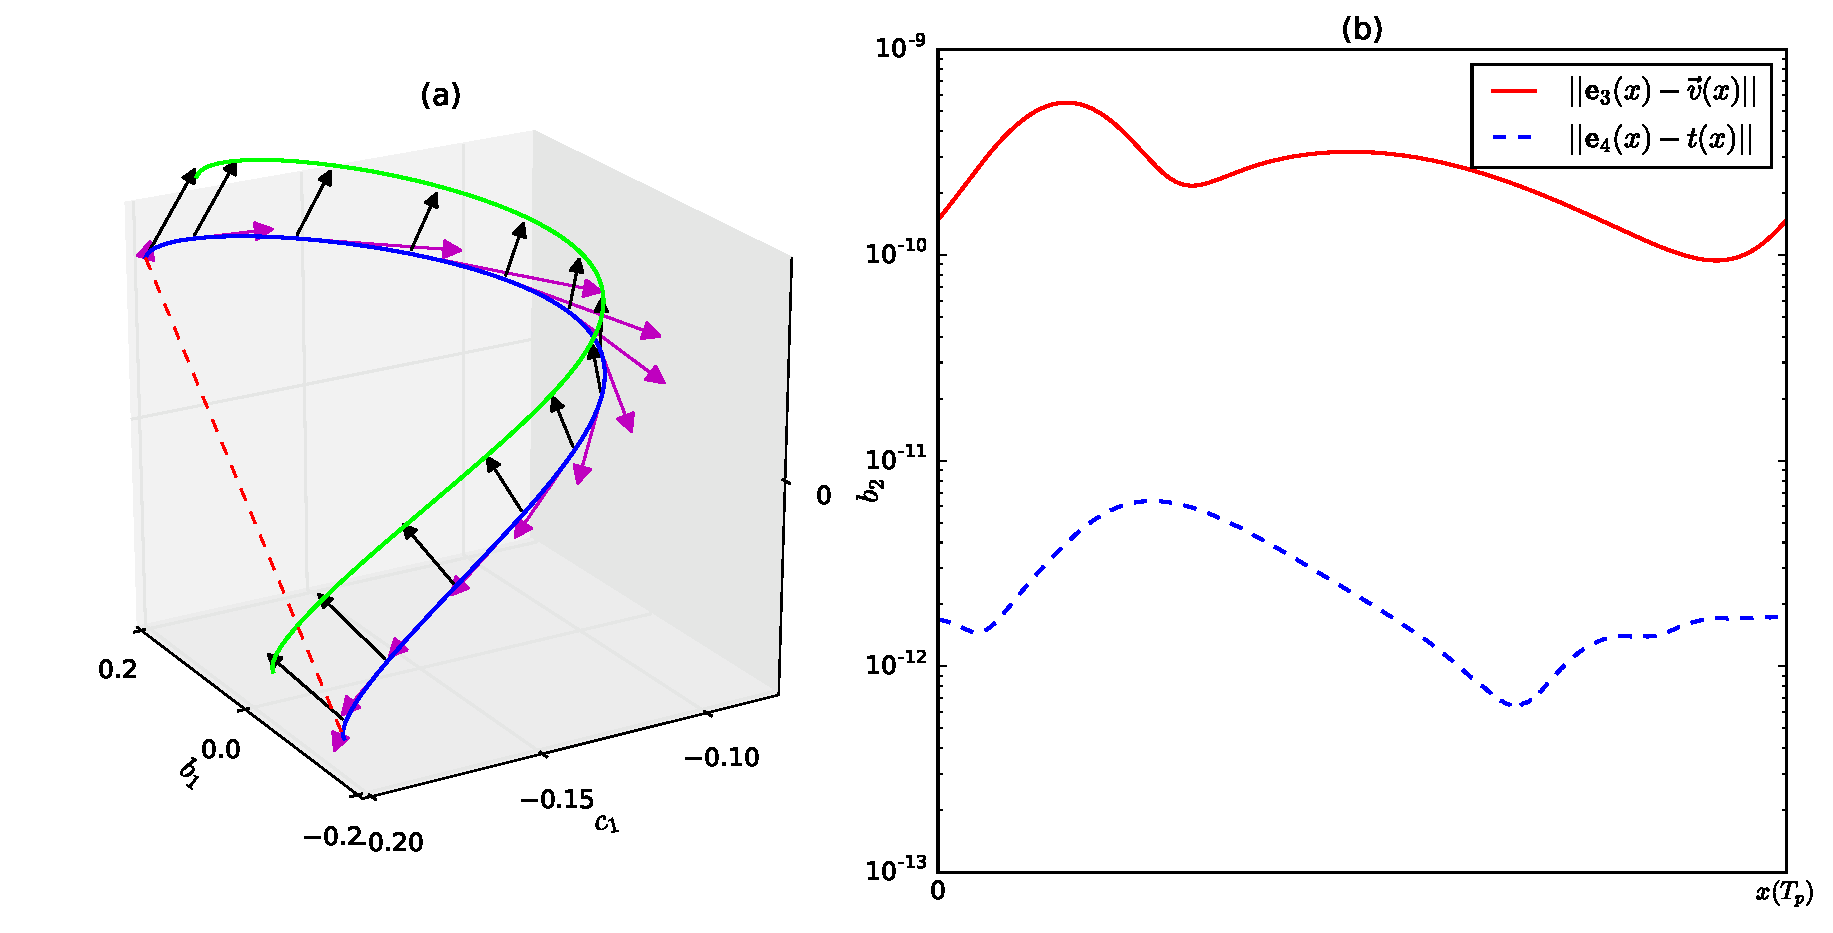
\includegraphics[width=1.0\linewidth]{ppo1vectfield}
  \caption[The accuracy of the two marginal vectors of \PPO{10.25}.]{
    %(Color online)
    Marginal vectors and the associated errors.
    (a) \PPO{10.25} in one period projected into
    {$[b_1, c_{1}, b_{2}]$}
    subspace (blue curve), and its counterpart (green line) generated by
    a small group transformation $\LieEl(\gSpace)$
    , here arbitrarily set to $\gSpace= 0.1$. Magenta and black
    arrows represent the first and the second marginal \Fv s
    $\jEigvec[3](x)$ and $\jEigvec[4](x)$ along the prime orbit.
    (b) The solid red curve is the {Euclidean} difference between
    $\jEigvec[3](x)$ and the velocity field $\vel(x)$ along the orbit,
    and the blue dashed curve is the difference between $\jEigvec[4](x)$ and
    the group tangent $t(x)=\Lg x$.
  }
  \label{fig:ppo1vectorfield}
\end{figure}

The two marginal directions have a simple geometrical interpretation and provide
a metric for us to measure the convergence of \ped.
\refFig{fig:ppo1vectorfield}\,(a) depicts the two marginal vectors of
\PPO{10.25} projected into the subspace spanned
by {$[b_1, c_{1}, b_{2}]$}
(the real, imaginary parts of the first mode and the real part of the
second Fourier mode). The first marginal {direction} (the $3$rd
\Fv\ in  \reftab{tab:floquet_ppo1}) is aligned with the velocity
field along the orbit, and the second marginal direction (the $4$th
\Fv ) is aligned with the group tangent. The numerical
difference between the unit vectors along these two marginal directions
and the corresponding physical directions is shown in
\reffig{fig:ppo1vectorfield}\,(b). The difference is under $10^{-9}$ and
$10^{-11}$ for these two directions, which demonstrates the accuracy of
the algorithm.
As shown in \reftab{tab:floquet_ppo1}, for a pre\po, such as \PPO{10.25},
the {velocity field} and the group tangent have eigenvalue $+1$ and
$-1$ respectively, and are thus distinct. However, the two marginal
directions are degenerate for a \rpo, such as \RPO{16.31}. So these two
directions are not fixed, but the
two\dmn\ plane spanned by them is uniquely
determined. \refFig{fig:rpo1_marginal3} shows that the velocity field and
group tangent along orbit \RPO{16.31} indeed lie in the subspace spanned
by these two marginal directions.

\begin{figure}[h]
  \centering
  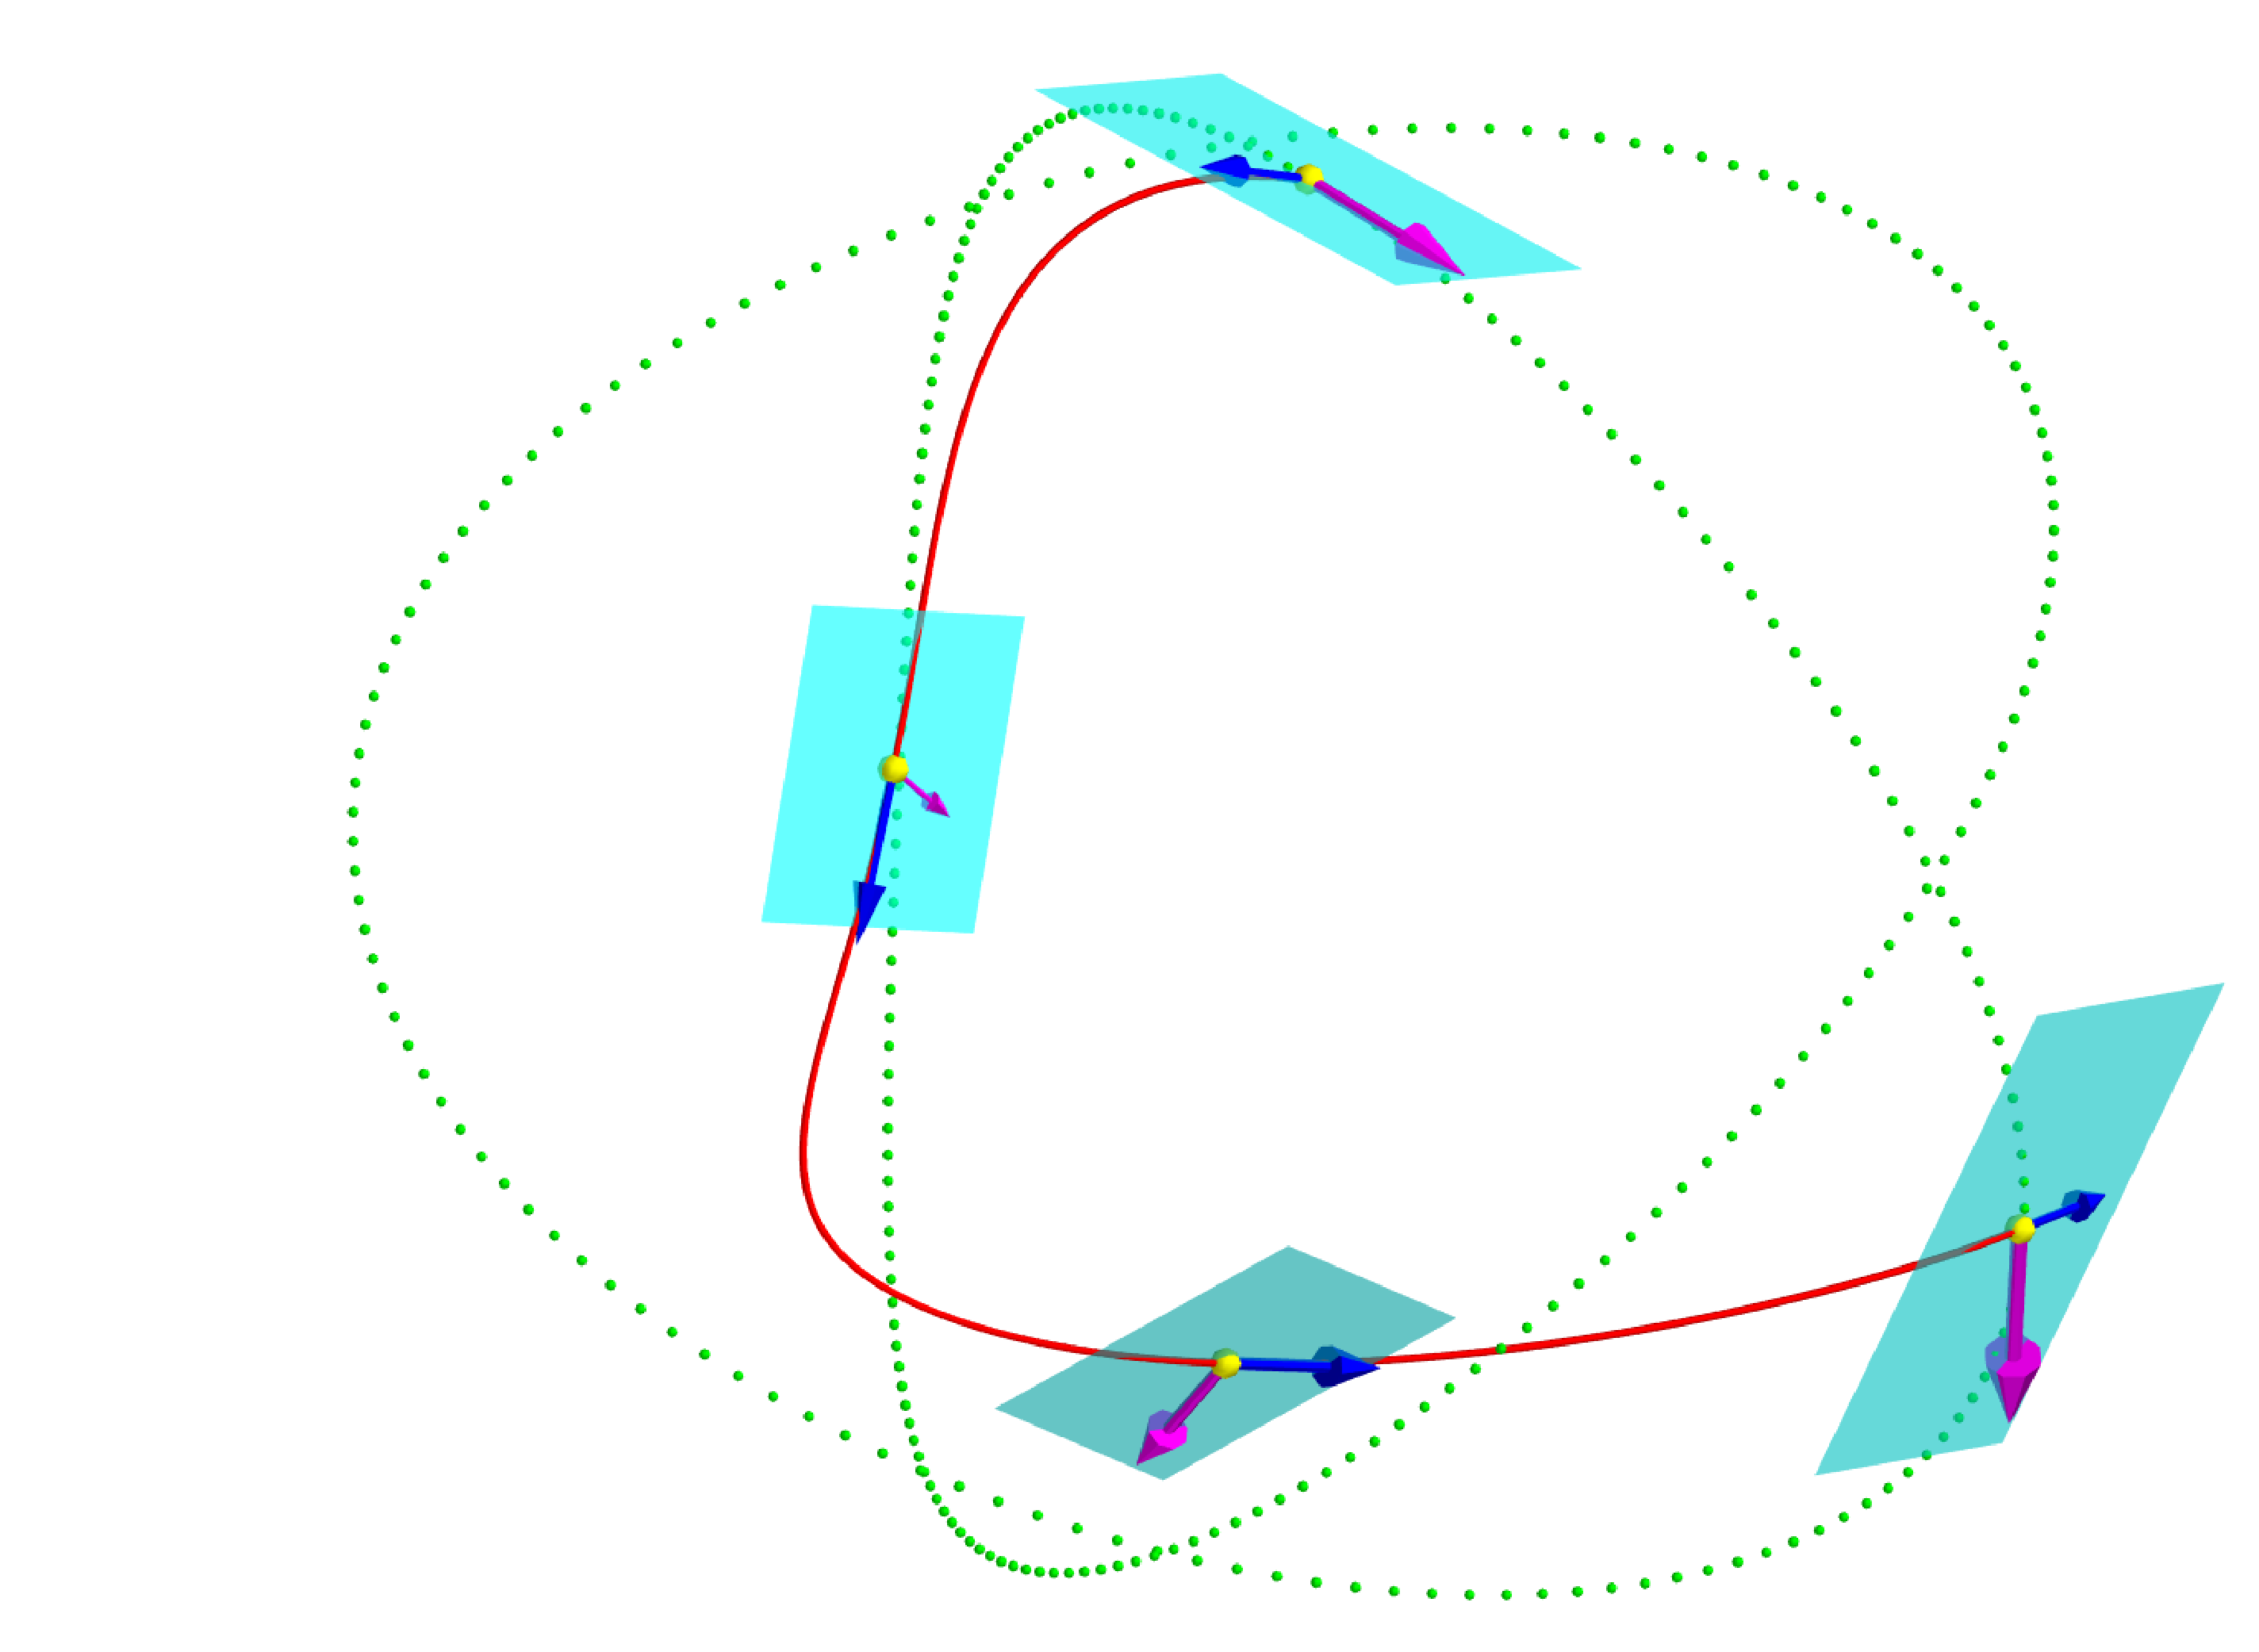
\includegraphics[width=0.7\linewidth]{rpo1_marginal3}
  \caption[The plane spanned by the two marginal vectors of \RPO{16.31}.]{
    %(Color online)
    Projection of \rpo\ \RPO{16.31} into
    the Fourier modes
    subspace $[b_2,c_2,b_3]$ (red curve). The dotted
    curve (lime) is the group orbit
    connecting the initial and final points. Blue and magenta arrows
    represent the velocity field and group tangent along the orbit,
    respectively. Two\dmn\ planes (cyan) are spanned by the
    two marginal \Fv s at each point (yellow) along the orbit.
  }
  \label{fig:rpo1_marginal3}
\end{figure}

\subsection{The choice of the number of orbit segments}

\begin{figure}[h]
  \centering
  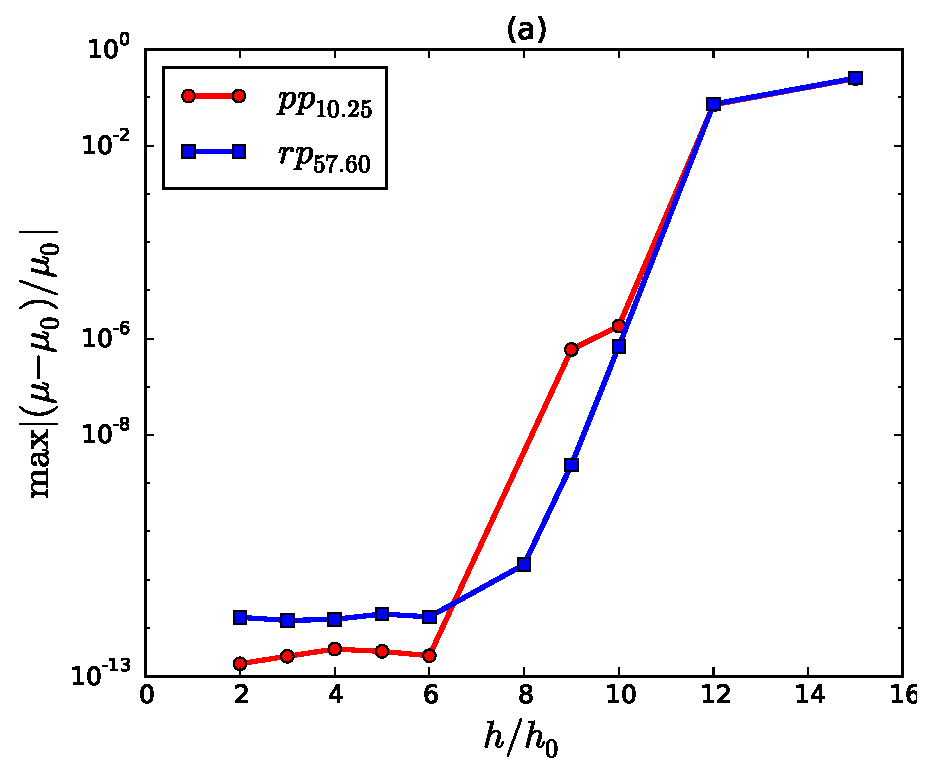
\includegraphics[width=0.47\linewidth]{ppo1FEerror} \hfill
  \includegraphics[width=0.47\linewidth]{rpo22FEerror}
  \caption[Accuracy of choosing different number of orbit segments]{
    %(Color online)
    Relative error of the real part of
    Floquet exponents associated with different time steps
    with which the Floquet matrix is integrated. Two orbits \PPO{10.25}
    and \RPO{57.60} are used as an example with the base
    case $h_0 \approx 0.001$. (a) The maximal relative difference of
    the whole set of Floquet exponents with increasing time step (decreasing
    the number of ingredient segments of the orbit). (b) Only consider
    the first 35 Floquet exponents.}
  \label{fig:FEerror}
\end{figure}


We have noted above that the {semi-group property of \JacobianM}
\eqref{eq:xjacobian} enables us to factorize
$\ps{\jMps}{k}$ into a product of short-time matrices with matrix
elements of comparable {order of magnitude}. In practice, caution should be
exercised when trying to determine the optimal number of time increments
that the orbit should be divided into. If the number of time increments
$m$ is too large, then, according to the estimates of
\refsect{sect:error}, the computation may be too costly. If $m$ is too
small, then the elements of the \JacobianM\ corresponding to the
corresponding time increment may range over too many orders of magnitude,
causing \ped\ to fail to resolve the most contracting \Fv\
along the orbit. One
might also vary the time step according to the velocity at a given point
on the orbit. Here we determined satisfactory $m$'s by numerical
experimentation shown in \reffig{fig:FEerror}. Since larger time step means
fewer time increments of the orbit, a very small time step ($h_0 \approx 0.001$)
is chosen as the base case, and it is increased to test whether the
corresponding Floquet exponents change substantially or not. As shown in
\reffig{fig:FEerror} (a), up to $6h_0$ the whole Floquet spectrum varies within
$10^{-12}$ for both \PPO{10.25} and $\cycle{rp}_{57.60}$. These
two orbits represent two different types of invariant solutions which have
short and long periods respectively,
so we presume that time step $6h_0$ is good enough
for other short or long orbits too. On the other hand, if only the first
few Floquet exponents are desired, the time step can be increased further
to fulfill the job. As shown in \reffig{fig:FEerror} (b), if we are only
interested in the first 35 Floquet exponents, then time step $30h_0$ is small
enough. In high\dmn\ nonlinear systems, often we are not interested in
very contraction
directions because dynamics in these directions are transient and shed little
insight into the system properties. Therefore, large time step could be used to
save time.




\section{Conclusion and future work}
\label{sect:concl}

In this chapter
we have used the one\dmn\ \KS\ system to illustrate the effectiveness
of \ped\ applied to stability analysis
in dissipative nonlinear systems.
In future, we hope to apply the method to
the study of orbits of much longer
periods, as well as to the study of high\dmn\, numerically exact
time-recurrent unstable solutions of the full \NS\ equations.
We anticipate the need for
optimizing and parallelizing such algorithms.
Also, if \ped\ is to be applied to Hamiltonian systems, additional
adjustments will be required to guarantee the preservation of symmetries
of Floquet spectrum imposed by the symplectic structure of Hamiltonian
flows.
